

\documentclass{beamer}



\mode<presentation>
{
  \usetheme{Frankfurt}
  % or ...

  %\setbeamercovered{transparent}
  % or whatever (possibly just delete it)
}
\usepackage[slovene]{babel}
\usepackage[utf8]{inputenc}
%\usepackage[pdftex]{graphicx}
%\usepackage{color}
%\usepackage{float}
%\usepackage{eurosym}

\usepackage{amsfonts}
\usepackage{amsmath,amsthm}
\usepackage{url}

%\usepackage[english]{babel}
% or whatever

%\usepackage[latin1]{inputenc}
% or whatever

%\usepackage{beamerthemeshadow}
\usepackage{times}
%\usepackage[T1]{fontenc}
% Or whatever. Note that the encoding and the font should match. If T1
% does not look nice, try deleting the line with the fontenc.

\newcommand{\bx}{\mathbf{x}}
\DeclareMathOperator{\Gl}{Gl}
\DeclareMathOperator{\adj}{adj}
%\newcommand{\Gl}{{\mathrm {GL}}\,}
%\newizrek{proposition}[izrek]{Proposition}

% finan�ni instrumenti
\newcommand{\PV}{\mathrm{PV}}


\newcommand{\ds}{\displaystyle}
\newcommand{\ts}{\textstyle}
\newcommand{\presledek}{\vspace{3mm}}
\newcommand{\ph}{\phantom{1}} % pomoč pri poravnavi teksta v slikah TikZ


\newcommand{\abs}[1]{ \left\lvert#1\right\rvert} 
\newcommand{\norm}[1]{\left\lVert#1\right\rVert}
\newcommand{\Co}{\operatorname{Co}} %konveksna ogrinjača

\newcommand{\R}{\mathbb R}
\newcommand{\N}{\mathbb N}
\newcommand{\Z}{\mathbb Z}
\newcommand{\C}{\mathbb C}
\newcommand{\Q}{\mathbb Q}
\newtheorem{izrek}{Izrek}
\newtheorem{lema}[izrek]{Lema}
\newtheorem{trditev}[izrek]{Trditev}
\newtheorem{posledica}[izrek]{Posledica}
\newtheorem{definicija}[izrek]{Definicija}
\newtheorem{naloga}[izrek]{Naloga}
\newtheorem{resitev}[izrek]{Naloga}
\setbeamertemplate{lema}[numbered]
\newcounter{saveenumi}
\newcommand{\seti}{\setcounter{saveenumi}{\value{enumi}}}
\newcommand{\conti}{\setcounter{enumi}{\value{saveenumi}}}
\resetcounteronoverlays{saveenumi}


\title[Računanje izotropnih vektorjev] % (optional, use only with long paper titles)
{Računanje izotropnih vektorjev}

%\subtitle
%{Presentation Subtitle} % (optional)

\author[Mirjam Pergar] % (optional, use only with lots of authors)
{\textbf{Avtor:}  Mirjam Pergar\\
\textbf{Mentor:} prof. dr. Bor Plestenjak
}
% - Use the \inst{?} command only if the authors have different
%   affiliation.

\institute[Fakuleta za matematiko in fiziko] % (optional, but mostly needed)
% \inst{FMF}
%

%  \and
%  \inst{2}%
%  Department of Theoretical Philosophy\\
%  University of Elsewhere

% - Use the \inst command only if there are several affiliations.
% - Keep it simple, no one is interested in your street address.

\date[16. maj 2016] % (optional)
{16. maj 2016}

\subject{Talks}
% This is only inserted into the PDF information catalog. Can be left
% out.



% If you have a file called "university-logo-filename.xxx", where xxx
% is a graphic format that can be processed by latex or pdflatex,
% resp., then you can add a logo as follows:

% \pgfdeclareimage[height=0.5cm]{university-logo}{university-logo-filename}
% \logo{\pgfuseimage{university-logo}}



% Delete this, if you do not want the table of contents to pop up at
% the beginning of each subsection:
%\AtBeginSubsection[]
%{
%  \begin{frame}<beamer>
%    \frametitle{Outline}
%    \tableofcontents[currentsection,currentsubsection]
%  \end{frame}
%}


% If you wish to uncover everything in a step-wise fashion, uncomment
% the following command:

%\beamerdefaultoverlayspecification{<+->}
\setbeamertemplate{footline}[frame number]

\begin{document}

\begin{frame}
  \titlepage
\end{frame}

\begin{frame}
  \frametitle{Vsebina}
  \tableofcontents
  % You might wish to add the option [pausesections]
\end{frame}


\section{Uvod}
\subsection{Problem}
\begin{frame}
  \frametitle{Problem}
\begin{alertblock}{}
Naj bo $A\in\R^{n\times n} (\C^{n\times n})$, $det(A)\ne 0$. Iščemo enotski vektor $b$, da je
\begin{equation}\label{eq:zac}
b^\ast Ab=0
\end{equation}
pravimo mu \textbf{izotropni vektor}. \medskip \\
Bolj splošen je inverzni problem numeričnega zaklada, kjer iščemo enotski vektor $b$, za katerega velja:
\begin{equation}\label{eq:splosno}
b^\ast Ab=\mu,
\end{equation}
kjer je $\mu \in \C$ dano število.
\end{alertblock}
\end{frame}
\begin{frame}
\begin{itemize}
\item Problem \eqref{eq:splosno} prevedemo na problem \eqref{eq:zac} za drugo matriko $ (A-\mu I)$.\medskip
\item Če $\mu$ lastna vrednost matrike $A$, potem je rešitev pripadajoč lastni vektor matrike $A$.\medskip
\item Če $\mu$ ni lastna vrednost matrike $A$, je $det(A-\mu I)\ne 0$ in je potreben izračun izotropnega vektorja te matrike.\medskip
\item Od sedaj naprej bomo vse vrednosti $\mu$ enačili z $0$.\medskip
\end{itemize}
\end{frame}
\begin{frame}
\frametitle{Numerični zakladi}
\begin{definicija}
\textbf{Numerični zaklad} matrike $A \in \C^{n\times n}$ je podmnožica kompleksne ravnine, definirana kot
$$W(A)=\{x^\ast Ax: x \in \C^n, x^\ast x=1\}.$$
\end{definicija}\pause
\begin{itemize}
\item Očitno je $W(A)$ množica vseh Rayleighovih kvocientov matrike $A$.
\item $0 \in W(A)$, če hočemo, da ima \eqref{eq:zac} vsaj eno rešitev.
\item Označimo s $\sigma(A)$ množico vseh lastnih vrednosti matrike A, ki jo imenujemo spekter.
\end{itemize}
\end{frame}
\begin{frame}
\frametitle{Lastnosti numeričnega zaklada}
\begin{enumerate}[1.]
\item $W(A)$ je konveksen, zaprt in omejen.
\item $\sigma(A)\subseteq W(A).$
\item Za vsako unitarno matriko $U$ je $W(U^\ast AU)=W(A).$
\item $W(A+zI)=W(A)+z$ in $W(zA)=zW(A)$ za vsako kompleksno število $z$.
\item Rob $W(A), \partial W(A)$, je kosoma algebrska krivulja, in vsaka točka, v kateri $\partial W(A)$ ni diferenciabilen, je lastna vrednost matrike $A$.
\item Če je $A$ normalna, potem $W(A)=\Co(\sigma(A))$, kjer s $\Co$ označimo zaprto konveksno ogrinjačo množice.
\item $W(A)$ je daljica na realni osi, če in samo če je $A$ hermitska.
\end{enumerate}
\end{frame}
\begin{frame}
\begin{izrek}
Naj bo $A\in\R^{n\times n} (\C^{n\times n})$ in $b\in\R^n(\C^n)$.  Potem veljajo enakosti:
$$b^\ast Ab=0\Leftrightarrow b^\ast (A+A^\ast)b=0 \quad \text{in}\quad  b^\ast(A-A^\ast)b=0.$$
\end{izrek}\pause
%\begin{proof}
%($\Rightarrow$) Če velja $b^\ast Ab=0$, je tudi $(b^\ast Ab)^\ast=b^\ast A^\ast b=0$. Preoblikujemo prvo enačbo na desni v $b^\ast Ab +b^\ast A^\ast b$ dobimo 0. Drugo enačbo dokažemo na podoben način.\\
%($\Leftarrow$) S seštevkom enačb na desni dobimo enačbo na levi:
%\begin{align*}
% b^\ast (A+A^\ast)b+b^\ast(A-A^\ast)b=0\\
%b^\ast (2A)b=0\\
%b^\ast Ab=0
%\end{align*}
%\end{proof}
%\end{frame}
%\begin{frame}
\begin{itemize}
\item Če velja le $b^\ast (A+A^\ast)b=0 \Rightarrow \Re(b^\ast Ab)=0$.
\item Če velja le $b^\ast(A-A^\ast)b=0 \Rightarrow \Im(b^\ast Ab)=0$.
\item Označimo z $A_{sim}=(A+A^T)/2$ simetrični del matrike $A$.
\item Z $A_{psim}=(A-A^T)/2$ pa poševno-simetrični del matrike $A$.
\item Hermitski del matrike $A$ bomo označili s $H=(A+A^\ast)/2$.
\item Poševno-hermitski del matrike $A$ bomo označili z \medskip$\tilde{K}=(A-A^\ast)/2=\imath K$.
\end{itemize}
%\begin{proof}
%To sledi iz $b^T Ab=b^T A_{sim} b +b^T A_{psim} b=b^T A_{sim} b,$ kjer je z $A_{sim}$ označen simetrični del matrike $A$  in z $A_{psim}$ poševno-simetrični del matrike A.
%\end{proof}
\end{frame}
%\begin{frame}
%\begin{itemize}
%\item Hermitski del matrike $A$ bomo označili s $H=(A+A^\ast)/2$.
%\item Poševno-hermitski del matrike $A$ bomo označili z $\tilde{K}=(A-A^\ast)/2=\imath K$.
%\end{itemize}
%\end{frame}
\subsection{Uporaba}
\begin{frame}
\frametitle{Uporaba}
\begin{itemize}
\item Preučevanje konvergence nekaterih iterativnih metod za reševanje linearnih sistemov, npr. GMRES.\medskip
\item Aplikacije v numerični analizi, diferencialnih enačbah, teoriji sistemov itd.
\end{itemize}
\end{frame}
\section{Realne matrike} %REALNE MATRIKE
\subsection{Uvod}
\begin{frame}
\frametitle{Realne matrike}
\begin{block}{}
Ko je $A\in\R^{n\times n}$ nas zanima, kako se izračuna rešitev enačbe:
\begin{equation}\label{eq:realna}
b^\ast Hb=0,
\end{equation}
kjer je $H\in\R^{n\times n}$ simetrična matrika (t.j. $H=H^T$).
\end{block}\pause
\begin{lema} %\cite{lipkin}
Izotropni vektorji matrike A so identični izotropnim vektorjem njenega simetričnega dela.
\end{lema} \pause
%Velja enakost:
%\begin{block}{}
%$$b^T Ab=0 \Leftrightarrow b^T (A+A^T)b=0.$$ 
%\end{block}\pause
Vemo:
\begin{itemize}
\item $W(A)$ je simetričen glede na realno os.
\item $0 \in W(A)$, če in samo če $\lambda_n\le0\le\lambda_1$, kjer sta $\lambda_n$ in $\lambda_1$ najmanjša in največja lastna vrednost matrike $H$.
\end{itemize}
\end{frame}
\begin{frame}
Naj bosta $x_1, x_n \in \R^n$ lastna vektorja, pripadajoča $\lambda_1$ in $\lambda_n$. Potem sta:
\begin{itemize}
\item $x_1^T Ax_1=x_1^T Hx_1=\lambda_1$,
\item $x_n^T Ax_n=x_n^T Hx_n=\lambda_n$
\end{itemize}
realni točki na skrajni levi in skrajni desni $W(A)$ na realni osi.
\begin{itemize}\pause
\item Realne rešitve \eqref{eq:realna} izračunamo z uporabo lastnih vektorjev matrike $H$. 
\item Predpostavimo, da iščemo vektorje $b$ z normo 1.
\item $H$ zapišemo kot $$H=X\Lambda X^T,$$ kjer je $\Lambda=\lambda_i I$ in $X$ je ortogonalna matrika lastnih vektorjev, tako da $X^T X=I$.
\end{itemize}
\end{frame}
\begin{frame}
\begin{itemize}
\item Uporabimo ta spektralni razcep v \eqref{eq:realna}: $$b^\ast Hb=b^\ast X\Lambda X^T b=0.$$ 
\item  Označimo s $c=X^Tb$ vektor projekcije $b$ na lastne vektorje matrike $H$. 
\end{itemize}\pause
\begin{izrek} \label{izrek2}
Naj bo $b$ rešitev problema \eqref{eq:realna}. Potem vektor $c=X^T b$ s komponentami $c_i$ zadošča naslednjima enačbama:
\begin{align}
\sum_{i=1}^{n} \lambda_i \abs{c_i}^2=0 \label{eq:en1},\\
\sum_{i=1}^{n}\abs{c_i}^2=1. \label{eq:en2}
\end{align}
\end{izrek}
\end{frame}
%\begin{frame}
%\begin{proof}
%Enačbo \eqref{eq:en1}  dokažemo tako, da $c=X^Tb$ oz. $c^\ast =b^\ast X$ vstavimo v \eqref{eq:realna} in dobimo $$b^\ast Hb=b^\ast X\Lambda X^T b= c^\ast \Lambda c=0.$$ Ker je $\Lambda$ diagonalna matrika, lahko $c^\ast \Lambda c$ zapišemo kot vsoto komponent $\bar{c_i}\lambda_i c_i=\lambda_i\abs{c_i}^2$, ko $i=1,2,...n$.
%Za enačbo \eqref{eq:en2} vemo, da je $\norm{b}_2=1$. Če normo zapišemo s $c$ dobimo $$\norm{b}_2=\norm{Xc}_2=\norm{c}_2=1,$$ saj je $X$ ortogonalna matrika.
%\end{proof}
%\end{frame}
\subsection{Iskanje izotropnih vektorjev}
\begin{frame}
\frametitle{Iskanje izotropnih vektorjev}
\begin{block}{}
Če niso vse lastne vrednosti H enako predznačene, potem mora za najmanjšo veljati $\lambda_n <0$. \medskip \\
 Naj bo $k<n$ tak, da je $\lambda_k >0$ in $0<t<1, t\in \R$ . Izberemo \medskip taka $c_n$ in $c_k$, da velja  $\abs{c_n}^2 =t$, $\abs{c_k}^2=1-t$ in $c_i =0$, $i\not=n,k$, \medskip  ker velja enačba $\sum_{i=1}^{n}\abs{c_i}^2=1$ ($t+ (1-t)=1$). Iz \medskip $\sum_{i=1}^{n} \lambda_i \abs{c_i}^2=0$ mora veljati enačba: $$\lambda_n t +\lambda_k (1-t)=0,$$ katere rešitev je:
\begin{equation*}
t_s=\frac{\lambda_k}{\lambda_k -\lambda_n}.
\end{equation*}
\end{block}
\end{frame}
\begin{frame}
\begin{itemize}
\item Absolutna vrednost $c_n$ (oz. $c_k$) je kvadratni koren od $t_s$ (oz. $1-t_s$).
\item Ker je $b=Xc$, sta realni rešitvi: $$b_1=\sqrt{t_s}x_n +\sqrt{1-t_s}x_k,\quad b_2=-\sqrt{t_s}x_n+\sqrt{1-t_s}x_k,$$ kjer sta $x_n$ in $x_k$ lastna vektorja pripadajoča  $\lambda_n$ in $\lambda_k$.\pause
\item Ker imata izraza v rešitvah enaka imenovalca, lahko rešitvi zapišemo kot: $$b_1=\sqrt{\lambda_k}x_n+\sqrt{\abs{\lambda_n}}x_k, \quad b_2=-\sqrt{\lambda_k}x_n+\sqrt{\abs{\lambda_n}}x_k$$.\pause
%(sledi iz \cite{lipkin}).
\item Vektor mora biti normiran:
\begin{align*}
b_1=\sqrt{\frac{\lambda_k}{\lambda_k +\abs{\lambda_n}}}x_n + \sqrt{\frac{\abs{\lambda_n}}{\lambda_k +\abs{\lambda_n}}}x_k,\\ b_2=-\sqrt{\frac{\lambda_k}{\lambda_k +\abs{\lambda_n}}}x_n + \sqrt{\frac{\abs{\lambda_n}}{\lambda_k +\abs{\lambda_n}}}x_k.
\end{align*}
\end{itemize}
% Konstruirani rešitvi sta neodvisni in še več, ortogonalni, če $\lambda_k =-\lambda_n$. 
\end{frame}
\begin{frame}
\frametitle{Število rešitev}
Če uporabimo vsak par pozitivnih in negativnih lastnih vrednosti, lahko postopek vrne toliko rešitev kot je dvakratno število parov lastnih vrednosti matrike $H$ z nasprotnimi predznaki, če so vse lastne vrednosti različne.\medskip \\ Naj bo $b\in\R^n$.\pause
\begin{posledica}%\cite{lipkin}
Dobljena izotropna vektorja sta ortogonalna ($b_1 ^T b_2=0$), če in samo če $\lambda_k=-\lambda_n$.
\end{posledica}
%\begin{proof}%gleda wi kot negativno, mi pa mamo abs
%$$b_1 ^T b_2=(\sqrt{\lambda_k}x_n+\sqrt{\abs{\lambda_n}}x_k)^T (-\sqrt{\lambda_k}x_1+\sqrt{\abs{\lambda_n}}x_k )= -(\lambda_n +\lambda_k).$$
%\end{proof}
\end{frame}
\begin{frame}
\frametitle{Neskončno rešitev}
Ko sta $A\in\R^{n\times n}$ in $b\in\R^n$ smo dokazali naslednji izrek: \medskip
\begin{izrek}
Če je $A\in\R^{n\times n}$ nedefinitna (t.j. ni pozitivno in negativno definitna), potem obstajata najmanj dva neodvisna realna izotropna vektorja.
\end{izrek}\pause \medskip

Pokazati želimo, da imamo neskončno število realnih rešitev in jih izračunati. 
%\item  Vzeti moramo vsaj tri različne lastne vrednosti, ki ne smejo biti istega predznaka (ko obstajajo).

\end{frame}
\begin{frame}
\begin{itemize}
\item Predpostavimo, da $\lambda_1 <0<\lambda_2<\lambda_3$.\pause
\item Naj bo $t_1=\abs{c_1}^2$, $t_2=\abs{c_2}^2$.\pause
\end{itemize}
Veljati mora enačba \eqref{eq:en2}
\begin{block}{}
\begin{equation*}%\label{trije}
\lambda_1 t_1 +\lambda_2 t_2 +\lambda_3 (1- t_1 -t_2)=0
\end{equation*} oz.
\begin{equation*}
(\lambda_1 -\lambda_3)t_1 +(\lambda_2 -\lambda_3)t_2 +\lambda_3=0,
\end{equation*}
s pogoji: $t_i \ge 0, i=1,2$ in $t_1 +t_2\le1$.
\end{block}{}
\end{frame}
\begin{frame}
\frametitle{Neskončno rešitev}
\begin{itemize}
\item Dobimo premico definirano v $(t_1,t_2)$ ravnini z enačbo:
\begin{block}{}
$$t_2=\frac{\lambda_3}{\lambda_3 - \lambda_2} -\frac{\lambda_3 -\lambda_1}{\lambda_3 -\lambda_2}t_1.$$
\end{block}\pause
\item Pogoji za $t_1,t_2$ definirajo trikotnik.
\item Preverimo, če premica seka trikotnik.
\item Vse dopustne vrednosti za $t_1$ in $t_2$ so dane z daljico v trikotniku. 
\item Zato obstaja neskončno število možnih pozitivnih parov $(t_1,t_2)$.
\end{itemize}
\end{frame}
\begin{frame}
\frametitle{Zgled}
Poglejmo si enostaven zgled za matriko $3x3$ z lastnimi \medskip vrednostmi $\lambda_1=-1, \lambda_2=1$ in $\lambda_3=2$.\medskip \\ Matrika lastnih vektorjev $X$ je enaka $I$.\medskip \\
%$A = \begin{bmatrix} 
%-1 & 0 & 0 \\ 
%0 &1 &0 \\ 
%0 &0 &2  
%\end{bmatrix}.$\\
%Očitno so lastne vrednosti $\lambda_1=-1, \lambda_2=1$ in $\lambda_3=2$. Drugače izračunamo lastne vrednosti in vektorje v Matlabu s pomočjo ukaza \texttt{[X,D] = eig(A)}. Kjer je $X$ matrika lastnih vektorjev in $D$ matrika lastnih vrednosti.
%$$X = \begin{bmatrix} 
%1 & 0 & 0 \\ 
%0 &1 &0 \\ 
%0 &0 &1  
%\end{bmatrix},$$
%$$D = \begin{bmatrix} 
%-1 & 0 & 0 \\ 
%0 &1 &0 \\ 
%0 &0 &2  
%\end{bmatrix}.$$
%\end{frame}
%\frametitle{Zgled}
Enačba premice je $t_2=2-3t_1$ s pogoji $t_1, t_2 \ge 0$ in $t_1+t_2\le 1$.
%\begin{center}
%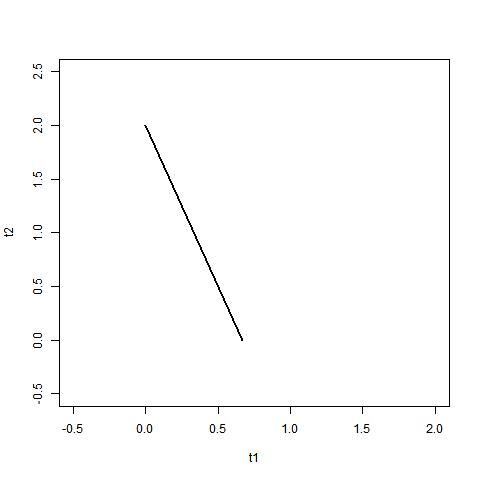
\includegraphics[width=7cm]{graf1.jpg}
%\end{center}
%\end{frame}
%\begin{frame}
%\frametitle{Zgled}
%Narišemo omejitve: $t_1, t_2 \ge 0$ in $t_1+t_2\le 1$.\pause
%\begin{center}
%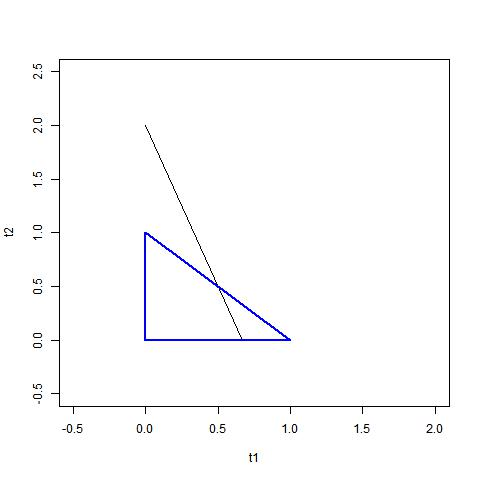
\includegraphics[width=7cm]{graf2.jpg}
%\end{center}
\end{frame}
\begin{frame}
\frametitle{Zgled}
Dopustne rešitve za $t_1$ in $t_2$ so dane z daljico v trikotniku.\pause
\begin{center}
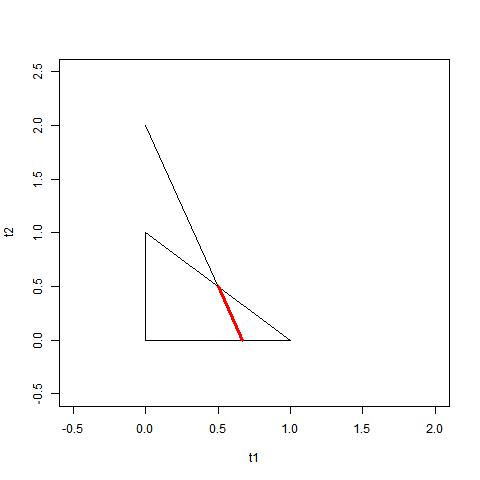
\includegraphics[width=7cm]{graf3.jpg}
\end{center}
\end{frame}
\begin{frame}
\frametitle{Zgled}
Iz daljice lahko izberemo katerikoli par točk $(t_1, t_2)$, npr. $(0.5, 0.5)$. Potem vemo kako izgleda vektor 
$c=\begin{bmatrix}
\sqrt{0.5}\\
\sqrt{0.5}\\
0
\end{bmatrix}$. Iz enačbe $c=X^T b$ dobimo 
$$b=Xc=c =\begin{bmatrix}
\sqrt{0.5}\\
\sqrt{0.5}\\
0
\end{bmatrix}.$$
Seveda je rešitev tudi $b=-c$. Tako dobimo neskončno izotropnih vektorjev $b$.
\end{frame}
\begin{frame}
\frametitle{Neskončno rešitev}
%Ta problem za iskanje koeficientov je v treh dimenzijah in možne rešitve $t$-ja so v eni dimenziji. 
Takšna konstrukcija pripelje do naslednjega izreka:
\begin{izrek}
Če je $n>2$ in je $A\in\R^{n\times n}$ nedefinitna, ima matrika $H$ vsaj tri različne lastne vrednosti z različnimi predznaki. Potem obstaja neskončno število realnih izotropnih vektorjev.
\end{izrek}\pause
\begin{block}{Splošen zapis}
\begin{equation*}
\sum_{i=1}^{k-1} (\lambda_i -\lambda_k)t_i +\lambda_k =0, \quad t_i\ge0,  i=1, \dots,k-1, \quad \sum_{i=1}^{k-1}t_i \le1.
\end{equation*}
\end{block}
\end{frame}
\section{Kompleksne matrike} %KOMPLEKSNE MATRIKE
\subsection{Uvod}
\begin{frame}
\frametitle{Kompleksne matrike}
Predstavljeni bodo algoritmi naslednjih avtorjev:\medskip
\begin{enumerate}[1.]
\item \emph{Meurant},
\item \emph{Carden},
\item \emph{Chorianopoulos, Psarrakos in Uhlig}.
\end{enumerate}\medskip
Algoritme bomo numerično primerjali, saj bi radi, da algoritem vrne izotropni vektor s čim manj računanja.
\end{frame}
\subsection{Meurant 1}
\begin{frame}
\frametitle{Meurant 1}
\begin{itemize}
\item V nekaterih primerih lahko izračunamo rešitve s samo enim ra\-ču\-na\-njem lastnih vrednosti in vektorjev matrike $K$, vendar to ne deluje vedno.
\item Uporabimo lastne vektorje matrike $H$.
\item Z uporabo treh lastnih vektorjev $H$, obstaja neskončno rešitev dobljenih na daljici v trikotniku omejitev.
\item  Če sta imaginarna dela, ki ustrezata robnima točkama daljice, različnih predznakov, potem iz izreka o povprečni vrednosti sledi, da obstaja točka na daljici, ki ima $\Im =0$.%ničeln imaginarni del.
\end{itemize}
\end{frame}
\subsection{Meurant 2}
\begin{frame}
\frametitle{Meurant 2}
\begin{itemize}
\item Uporabimo lastne vrednosti in lastne vektorje hermitske matrike $K=(A-A^\ast)/(2i)$.
\item S kombiniranjem lastnih vektorjev matrike $K$ pripadajočim k pozitivnim in negativnim lastnim vrednostim, lahko (v nekaterih primerih) izračunamo taka vektorja $b_1$ in $b_2$, da $$\alpha_1=\Re(b_1^\ast Ab_1)<0$$ in $$\alpha_2=\Re(b_2^\ast Ab_2)>0.$$
\end{itemize}
\end{frame}
\begin{frame}
\frametitle{Meurant 2}
\begin{lema}\label{komp}
Naj bosta $b_1$ in $b_2$ enotska vektorja z $\Im(b_i^\ast Ab_i)=0$, $i=1,2$ in \medskip $\alpha_1=\Re(b_1^\ast Ab_1)<0$,  $\alpha_2=\Re(b_2^\ast Ab_2)>0$. Naj bo $b(t,\theta)=e^{-i\theta}b_1 + tb_2$, $t, \theta \in \R$ in  $\alpha(\theta)=e^{i\theta}b_1^\ast Ab_2 +e^{-i\theta}b_2^\ast Ab_1.$ Potem je 
$$b(t,\theta)^\ast Ab(t,\theta)=\alpha_2 t^2 +\alpha(\theta)t+\alpha_1,$$ 
$\alpha(\theta)\in\R$, ko $\theta=arg(b_2^\ast Ab_1 -b_1^T\bar{A}\bar{b_2}).$\medskip \\ Za $t_1 =(-\alpha(\theta) +\sqrt{\alpha(\theta)^2 -4\alpha_1\alpha_2})/(2\alpha_2)$  imamo 
$$b(t_1, \theta) \not=0,\quad  \frac{b(t_1,\theta)^\ast}{\norm{b(t_1,\theta)}}A\frac{b(t_1,\theta)}{\norm{b(t_1,\theta)}}=0.$$
\end{lema}
\end{frame}
%\begin{frame}
%\frametitle{Meurant 2.}
%\begin{itemize}
%\item  Če imamo $b_1$ in $b_2$, taka da  $\alpha_1=\Re(b_1^\ast Ab_1)<0$ in $\alpha_2=\Re(b_2^\ast Ab_2)>0$, smo končali.
%\item  Ko je $A$ realna in imamo $b_1=x_1, b_2=x_2$ za lastne vektorje $H$, potem je $\theta=0$ in nam lema \ref{komp} pove, kako se izračuna en izotropni vektor.
%\item  V kompleksnem primeru, ne moremo vedno najti primernih vektorje $b_1$ in $b_2$.
%\item Konstrukcija ne deluje, če imajo vrednosti $\Re(y_i^\ast Hy_j)$ enak predznak, kjer so $y_i$ lastni vektorji $K.$
%\end{itemize}
%\end{frame}
\begin{frame}
\frametitle{Algoritem}
\begin{enumerate}[1.]
\item S kombiniranjem lastnih vektorjev $K$, pripadajočim pozitivnim in negativinim lastnim vrednostim, izračunamo taka $b_1$ in $b_2$, da  $\alpha_1=\Re(b_1^\ast Ab_1)<0$ in $\alpha_2=\Re(b_2^\ast Ab_2)>0$. Uporabimo lemo in končamo.\medskip
\item Če ne najdemo $b_1$, $b_2$ potrebna za lemo, izračunamo še lastne vektorje matrike $H$.  Ponovimo korak 1. za matriko $\imath A$.\medskip
\item Če postopek ne deluje niti za $\imath A$, uporabimo kombinacijo lastnih vektorjev $K$ in $H$, kjer z $x$ označimo lastni vektor $K$ in z $y$ lastni vektor $H$.\medskip
\item Upoštevamo vektorje $X_\theta =\cos(\theta)x+\sin(\theta)y$$, 0\le\theta\le\pi$. $X_\theta ^\ast AX_\theta$ opiše elipso znotraj $W(A)$.
\seti
\end{enumerate}
\end{frame}
\begin{frame}
\frametitle{Algoritem}
\begin{enumerate}[1.]
\conti
\item Za dan par $(x,y)$ iščemo presečišča elipse $X_\theta ^\ast AX_\theta$ z realno osjo. U\-po\-šte\-va\-mo, da je $A=H+iK$: 
\begin{align*}
X_\theta^\ast AX_\theta &= \cos^2(\theta)(x^\ast Hx + ix^\ast Kx)\\ 
&+ \sin^2(\theta)(y^\ast Hy + iy^\ast Ky)\\ 
&+\sin(\theta)\cos(\theta)(x^\ast Hy +y^\ast Hx +i[x^\ast Ky +y^\ast Kx]).
\end{align*}
Naj bo $\alpha=\Im(x^\ast Hx + ix^\ast Kx)$, $\beta=\Im(y^\ast hy +iy^\ast Ky)$ in\medskip $\gamma=\Im(x^\ast Hy +y^\ast Hx +i[x^\ast Ky +y^\ast Kx]).$ Ko izenačimo $\Im(X_\theta ^\ast AX_\theta)=0$, dobimo enačbo:
$$\alpha \cos^2(\theta) +\beta \sin^2(\theta) +\gamma \sin(\theta)\cos(\theta)=0.$$
Predpostavimo, da $\cos(\theta) \not =0$ in delimo, dobimo kvadratno enačbo za $t=\tan(\theta),$
$$\beta t^2 +\gamma t +\alpha =0.$$
\seti
\end{enumerate}
\end{frame}
\begin{frame}
\frametitle{Algoritem}
\begin{enumerate}[1.]
\conti
\item Če ima ta enačba realne rešitve, potem dobimo vrednosti $\theta$, ki nam vrnejo take vektorje $X_\theta$, da $\Im(X_\theta ^\ast AX_\theta)=0$.\medskip
\item Če tudi ta konstrukcija ne deluje, uporabimo algoritem CPU.
\end{enumerate}
Opombe:
\begin{itemize}
%\item  Če imamo $b_1$ in $b_2$, taka da  $\alpha_1=\Re(b_1^\ast Ab_1)<0$ in $\alpha_2=\Re(b_2^\ast Ab_2)>0$, smo končali.
\item  Ko imamo za $A\in \R^{n\times n}$ $b_1=x_1, b_2=x_2$ za lastne vektorje $H$, potem je $\theta=0$ in nam lema pove, kako se izračuna en izotropni vektor.
%\item  V kompleksnem primeru, ne moremo vedno najti primernih vektorje $b_1$ in $b_2$.
\item Konstrukcija ne deluje, če imajo vrednosti $\Re(y_i^\ast Hy_j)$ enak predznak, kjer so $y_i$ lastni vektorji $K.$
\item Ko je velikost problema velika, uporabimo samo lastne vektorje, ki pripadajo par najmanjšim in največjim lastnim vrednostim.
\end{itemize}
\end{frame}
\subsection{Carden}
\begin{frame}
\frametitle{Carden}
Vseeno je, če rešujemo splošen problem (\ref{eq:splosno}) ali problem (\ref{eq:zac}) za matriko $A-\mu I$.\pause
\begin{itemize}
\item Predpostavimo, da je $\mu$ v konveksni ogrinjači treh točk $\theta_i \in W(A)$, za katere smo lahko izračunali izotropne vektorje $b_i$. 
\item Konveksna ogrinjača $\theta_i$ je trikotnik (lahko je izrojen).
\item Radi bi, da je $\mu$ na daljici, ki ima take robne točke, da za njih vemo ali lahko izračuamo izotropne vektorje. BSŠ predpostavimo, da je $\theta_1$ ena od robnih točk te daljice. Za drugo robno točko vzamemo $w$, ki je presečišče daljice med $\theta_2$ in $\theta_3$ s premico, ki teče skozi $\theta_1$ in $\mu$.
\end{itemize}
\end{frame}
\begin{frame}
\frametitle{Carden}
\begin{itemize}
\item $w$ je konveksna kombinacija $\theta_2$ in $\theta_3$, zato mu lahko določimo pripadajoč izotropni vektor. Ker pa je $\mu$ konveksna kombinacija $w$ in $\theta_1$, lahko tudi njemu določimo izotropni vektor.
\end{itemize}
\begin{center}
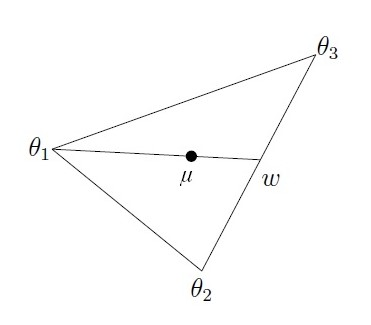
\includegraphics[width=5.5cm]{triangle.jpg}
\end{center}
\end{frame}
\begin{frame}
\frametitle{Algoritem}
Naj bo $\varepsilon >0$ (npr. $\varepsilon=10^{-16}\norm{A}$). 
\begin{enumerate}[1.]
\item Poiščemo zunanjo aproksimacijo $W(A)$, z izračunom najbolj leve in desne lastne vrednosti $H_\theta =(e^{i\theta}A+e^{-i\theta}A^\ast)/2$ za $\theta =0, \pi/2$. %S tem dobimo zunanjo aproksimacijo zaloge vrednosti, ki seka $\partial W(A)$ v robnih točkah. %RAZLAGA Zunanja aproksimacija bo pravokotnik, katerega stranice so vzporedne z realno in imaginarno osjo. 
Če $\mu$ ni v zunanji aproksimaciji, potem $\mu \not \in W(A)$ in ustavimo algoritem, drugače nadaljujemo.\medskip
\item Če je višina ali širina zunanje aproksimacije manj kot $\varepsilon$, potem je $W(A)$ približno hermitska ali poševno-hermitska in je $W(A)$ približno točka. Ugotovimo ali je $\mu \in W(A)$ in če je, poiščemo pripadajoč izotropni vektor. 
\seti
\end{enumerate}
\end{frame}
\begin{frame}
\frametitle{Algoritem}
\begin{enumerate}[1.]
\conti
\item Če $\mu \not \in W(A)$, nadaljujemo s konstrukcijo notranje aproksimacije $W(A)$ z uporabo lastnih vektorjev najbolj leve in desne lastne vrednosti $H_{\theta}$.\medskip% RAZLAGA Notranja aproksimacija bo štirikotnik z oglišči v robnih točkah $\partial W(A)$.
\item  Če $\mu$ leži v notranji aproksimaciji, lahko poiščemo izotropni vektor. %OPISS
Če $\mu$ ne leži v notranji aproksimaciji, določimo katera stranica notranje aproksimacije mu leži najbližje.\medskip
\item  Izračunamo $\hat{\mu}$, ki je najbližja točka do $\mu$, ki leži na notranji aproksimaciji. Če je $\abs{\hat{\mu}-\mu}<\varepsilon$, izračunamo izotropni vektor za $\hat{\mu}$ in ga sprejmemo kot izotropni vektor za $\mu$ ter ustavimo algoritem.
\seti
\end{enumerate}
\end{frame}
\begin{frame}
\frametitle{Algoritem}
\begin{enumerate}[1.]
\conti
\item Posodobimo notranjo in zunanjo aproksimacijo z izračunom največje lastne vrednosti in pripadajočega lastnega vektorja $H_{\theta}$, kjer je smer $\theta$ pravokotna na stranico notranje aproksimacije, ki je najbližja $\mu$. Če ne dobimo nove robne točke, ki se ni dotikala notranje aproksimacije, potem $\mu \not \in W(A)$. \medskip
\item Preverimo, če je $\mu$  v novi zunanji aproksimaciji. Če je, se vrnemo na 4. korak, drugače $\mu \not \in W(A)$. 
\end{enumerate}
\end{frame}
\begin{frame}
\frametitle{Algoritem}
Opombe: 
\begin{itemize}
\item Korake 4.-7. ponavljamo, dokler ni notranja aproksimacija $\varepsilon$ blizu $\mu$ ali dokler zunanja aproksimacija ne vsebuje $\mu$. Carden trdi, da se v večini primerov postopek konča v koraku 4. po le nekaj ponavljanjih.\\
\item Zunanja aproksimacija bo pravokotnik, katerega stranice so vzporedne z realno in imaginarno osjo.
\item Notranja aproksimacija pa štirikotnik z oglišči v robnih točkah $\partial W(A)$.
\end{itemize}
\end{frame}
\subsection{Chorianopoulos, Psarrakos in Uhlig}
\begin{frame}
\frametitle{Chorianopoulos, Psarrakos in Uhlig - CPU}
Ta algoritem naj bi bil hitrejši in dajal natančne numerične rezultate tam, kjer se prejšnja algoritma mnogokrat ustavita. Tak primer je ko:\medskip
\begin{itemize}
\item $\mu \in W(A)$ ali 
\item $\mu \not\in W(A)$ ali 
\item $\mu$ leži zelo blizu roba $\partial W(A)$. 
\end{itemize}
Ta algoritem uporabi za iskanje izotropnih vektorjev le nekaj najbolj osnovnih lastnosti numeričnega zaklada poleg konveksnosti, kot je $W(\alpha A +\beta I)=\alpha W(A) +\beta$.
\end{frame}
\begin{frame}
\frametitle{Algoritem}
\begin{enumerate}[1.]
\item Izračunamo do 4 robne točke $W(A)$, $p_i$ in njihove izotropne vektorje $b_i$ za $i=1,2,3,4$, tako da izračunamo ekstremne lastne vrednosti, ki pripadajo enotskim lastnim vektorjem $x_i$ matrike $H$ in $K$.\medskip
\item Nastavimo $p_i =b^\ast _i Ab_i$, ki jih označimo z $rM$ in $rm$ za maksimalen in minimalen horizontalen razteg $W(A)$ in z $iM$ in $im$ za maksimalen in minimalen vertikalen razteg $W(A)$.  Če je $|p_i|<10^{-13}$  za $i=1,2,3,4$, potem je naš izotropni vektor kar pripadajoč enotski vektor.\medskip
\item Če med računanjemi ugotovimo, da je ena od matrik $H$ in $iK$ definitna, potem vemo, da $\mu \not\in W(A)$, in algoritem ustavimo.
\seti
\end{enumerate}
\end{frame}\begin{frame}
\frametitle{Algoritem}
\begin{enumerate}[1.]
\conti
\item Narišemo elipse, ki gredo skozi vse možne pare točk $rm, rM, im$ in $iM$, ki imajo nasprotno predznačene imaginarne dele. Nato izračunamo presečišča vsake dobljene elipse z realno osjo\medskip.%Poiščemo presečišča realne osi z elipsami, ki so preslikave velikega kroga kompleksne sfere $\C^n$, %ko $x\mapsto x^\ast Ax$, ki grejo skozi vse možne pare izračunanih točk $p_i=x^\ast Ax$, $p_j=y^\ast  Ay$, tj. pari, ki imajo nasprotno predznačene imaginarne dele.
\item Če so izračunana presečišča na obeh straneh 0, potem izračunamo izotropni vektor z lemo.\medskip
\item Če presečišča niso na obeh straneh 0, potem moramo rešiti kvadratno enačbo s kompleksnimi števili
$$(tx +(1-t)y)^\ast A(tx+(1-t)y)  =$$
$$(x^\ast Ax+y^\ast Ay -(x^\ast Ay +y^\ast Ax))t^2 +$$
$$+(-2y^\ast Ay +(x^\ast Ay+y^\ast Ax))t +y^\ast Ay.$$
%Njene ničle določijo koordinatne osi $W(A)$ točk na elipsah skozi točke $x^\ast Ax$, $y^\ast Ay\in \partial W(A)$ %?????
%in so generirane s točkami v $\C^n$ na velikem krogu skozi $x$ in $y$. 
\seti
\end{enumerate}
\end{frame}\begin{frame}
\frametitle{Algoritem}
\begin{enumerate}[1.]
\conti
\item Zanimajo nas samo rešitve, ki imajo imaginaren del enak 0, saj želimo uporabiti lemo.
Če imaginarni del enačbe enačimo z 0, dobimo naslednjo polinomsko enačbo z realnimi koeficienti:
\begin{equation*}
t^2+gt+\frac{p}{f}=0 
\end{equation*}
za $q=\Im(x^\ast Ax)$, $p=\Im(y^\ast Ay)$ in $r=\Im(x^\ast  Ay + y^\ast Ax)$. Označimo $f=p+q-r$ in $g=(r-2p)/f$.\medskip
\item  Enačba ima realni rešitvi $t_i$, $i=1,2$, ki vrneta generirajoča vektorja $b_i=t_ix+(1-t_i)y$ ($i=1,2$) za realni točki. Z normalizacijo dobimo izotropne vektorje. %SLIKA
\seti
\end{enumerate}
\end{frame}\begin{frame}
\frametitle{Algoritem}
\begin{enumerate}[1.]
\conti
\item Če nobena od možnih elips ne seka realno os na vsaki strani 0, potem preverimo, če to stori njihova skupna množica in ponovimo isti postopek.\medskip
\item Če niti skupna množica ne gre, potem izračunamo še več lastnih vrednosti in lastnih vektorjev za $A(\theta)=\cos(\theta)H+\sin(\theta)iK$ za kote $\theta \not =0,\pi/2$ in delamo bisekcijo med točkami $rm$, $rM$, $im$, $iM$.\medskip
\item Končamo, ko najdemo definitno matriko $A(\theta)$ ali elipso, ki seka realno os na obeh straneh 0, nakar lahko uporabimo lemo.
\end{enumerate}
\end{frame}
\subsection{Primer}
\begin{frame}[fragile]
\frametitle{Primer}
Poglejmo si primer za algoritma Cardna in CPU za Matlabovo Grcar matriko $A$ s kompleksnim premikom $z$.
\begin{verbatim}
A=gallery('grcar',32);
z=1+3i;
\end{verbatim}
Uporabili bomo ukaza:
\begin{verbatim}
[bC no_eigC]=inversefov(A,z,0,10^-16,500)

[bCPU napaka no_eigCPU]=invfovCPU(A,z,1,1)
\end{verbatim}
\end{frame}
\begin{frame}[fragile]
\frametitle{Primer: Carden \texttt{inversefov}}

\begin{verbatim}
bC =

  -0.0065 - 0.0580i
   0.0554 - 0.0679i
   0.1132 - 0.0259i
   0.1368 + 0.0571i
   0.0887 + 0.1539i

no_eigC =

     5   

napakaC =

   2.3915e-15
\end{verbatim}
\end{frame}
\begin{frame}
\begin{center}
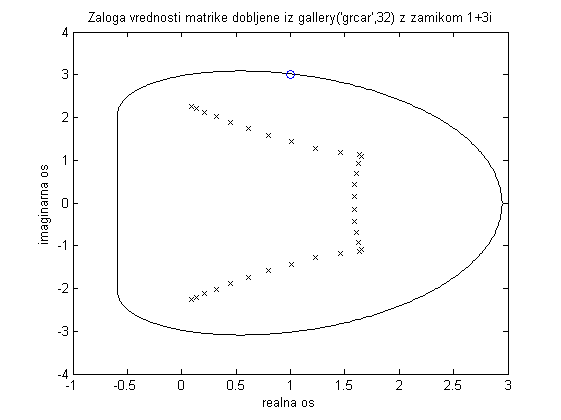
\includegraphics[width=11cm]{carden1.png}
\end{center}
\end{frame}
\begin{frame}
\begin{center}
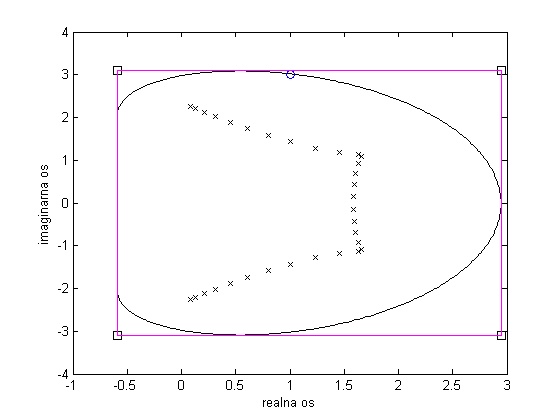
\includegraphics[width=11cm]{carden2.png}
\end{center}
\end{frame}
\begin{frame}
\begin{center}
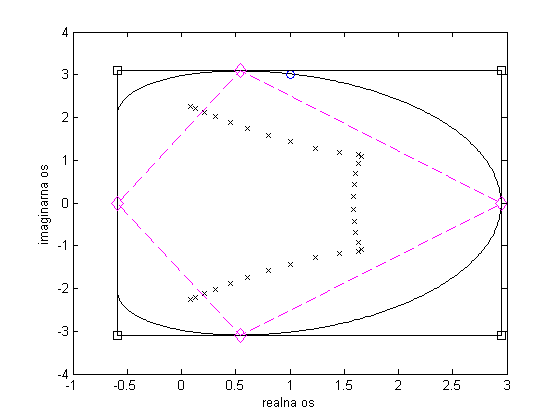
\includegraphics[width=11cm]{carden3.png}
\end{center}
\end{frame}

\begin{frame}[fragile]
\frametitle{Primer: CPU \texttt{invfovCPU}}
\begin{verbatim}
bCPU =

  -0.0271 - 0.0299i
  -0.0024 - 0.0610i
   0.0395 - 0.0704i
   0.0876 - 0.0530i
   0.1197 + 0.0032i

no_eigCPU =

     5

napaka =

   6.8450e-17
\end{verbatim}
\end{frame}
\begin{frame}
\begin{center}
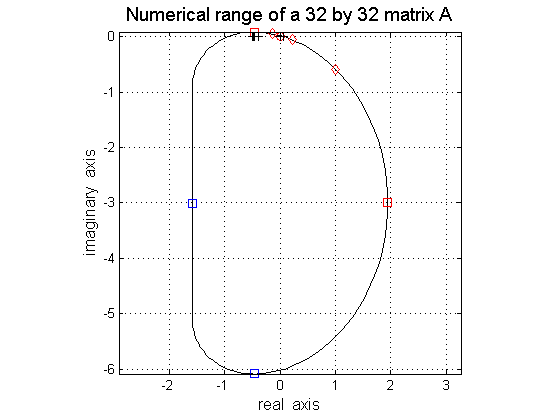
\includegraphics[width=11cm]{cpu1.png}
\end{center}
\end{frame}
\begin{frame}
\begin{center}
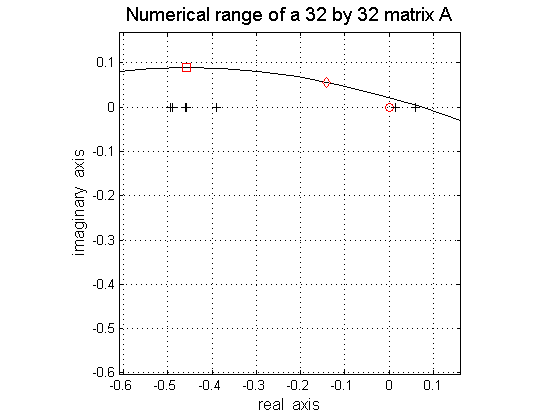
\includegraphics[width=11cm]{cpu2.png}
\end{center}
\end{frame}

\section{Literatura}
\begin{frame}
\frametitle{Literatura}
\begin{enumerate}
\item
G. Meurant, \emph{The computation of isotropic vectors}, Numer. Alg. {\bf 60} (2012) 193--204.
\item
R. Carden, \emph{A simple algorithm for the inverse field of values problem}, Inverse Probl. {\bf 25} (2009) 1--9
\item
C. Chorianopoulos, P. Psarrakos in F. Uhlig, \emph{A method for the inverse numerical range problem}, Electron. J. Linear Algebra {\bf 20} (2010) 198--206
\item
N. Ciblak, H. Lipkin, \emph{Orthonormal isotropic vector bases}, In: Proceedings of DETC'98, 1998 ASME Design Engineering Technical Conferences (1998).
\seti
\end{enumerate}
\end{frame}
\begin{frame}
\begin{enumerate}
\conti
\item
Johnson, C. R., \emph{Numerical determination of the field of values of a general complex matrix}, SIAM J. Numer. Anal. {\bf15} (1978) 595--602.
\item 
R. Carden, \emph{\texttt{inversefov.m}}, verzija 6.~2.~2011, [ogled 5.~5.~2016], dostopno na \url{http://www.caam.rice.edu/tech_reports/2009/}.
\item 
F. Uhlig, \emph{\texttt{invfovCPU.m}}, verzija 22.~3.~2011, [ogled 5.~5.~2016], dostopno na \url{http://www.auburn.edu/~uhligfd/m_files/invfovCPU.m}.
\end{enumerate}
\end{frame}
\end{document}

